\subsubsection{Thiết kế cơ sở dữ liệu}
\subsubsubsection{Thiết kế ý niệm}
Mục tiêu chính của phần này là xây dựng một mô hình dữ liệu trừu tượng, độc lập với các hệ quản trị cơ sở dữ liệu (DBMS) cụ thể, nhằm phản ánh chính xác các đối tượng dữ liệu và mối quan hệ giữa chúng trong hệ thống. Nhóm sử dụng mô hình Thực thể kết hợp mở rộng (EERD - Enhanced Entity-Relationship Diagram) để trực quan hóa cấu trúc thông tin, đảm bảo tính toàn vẹn và đáp ứng đầy đủ các chức năng cốt lõi của ứng dụng

\begin{landscape}
\begin{figure}[htp]
    \centering
    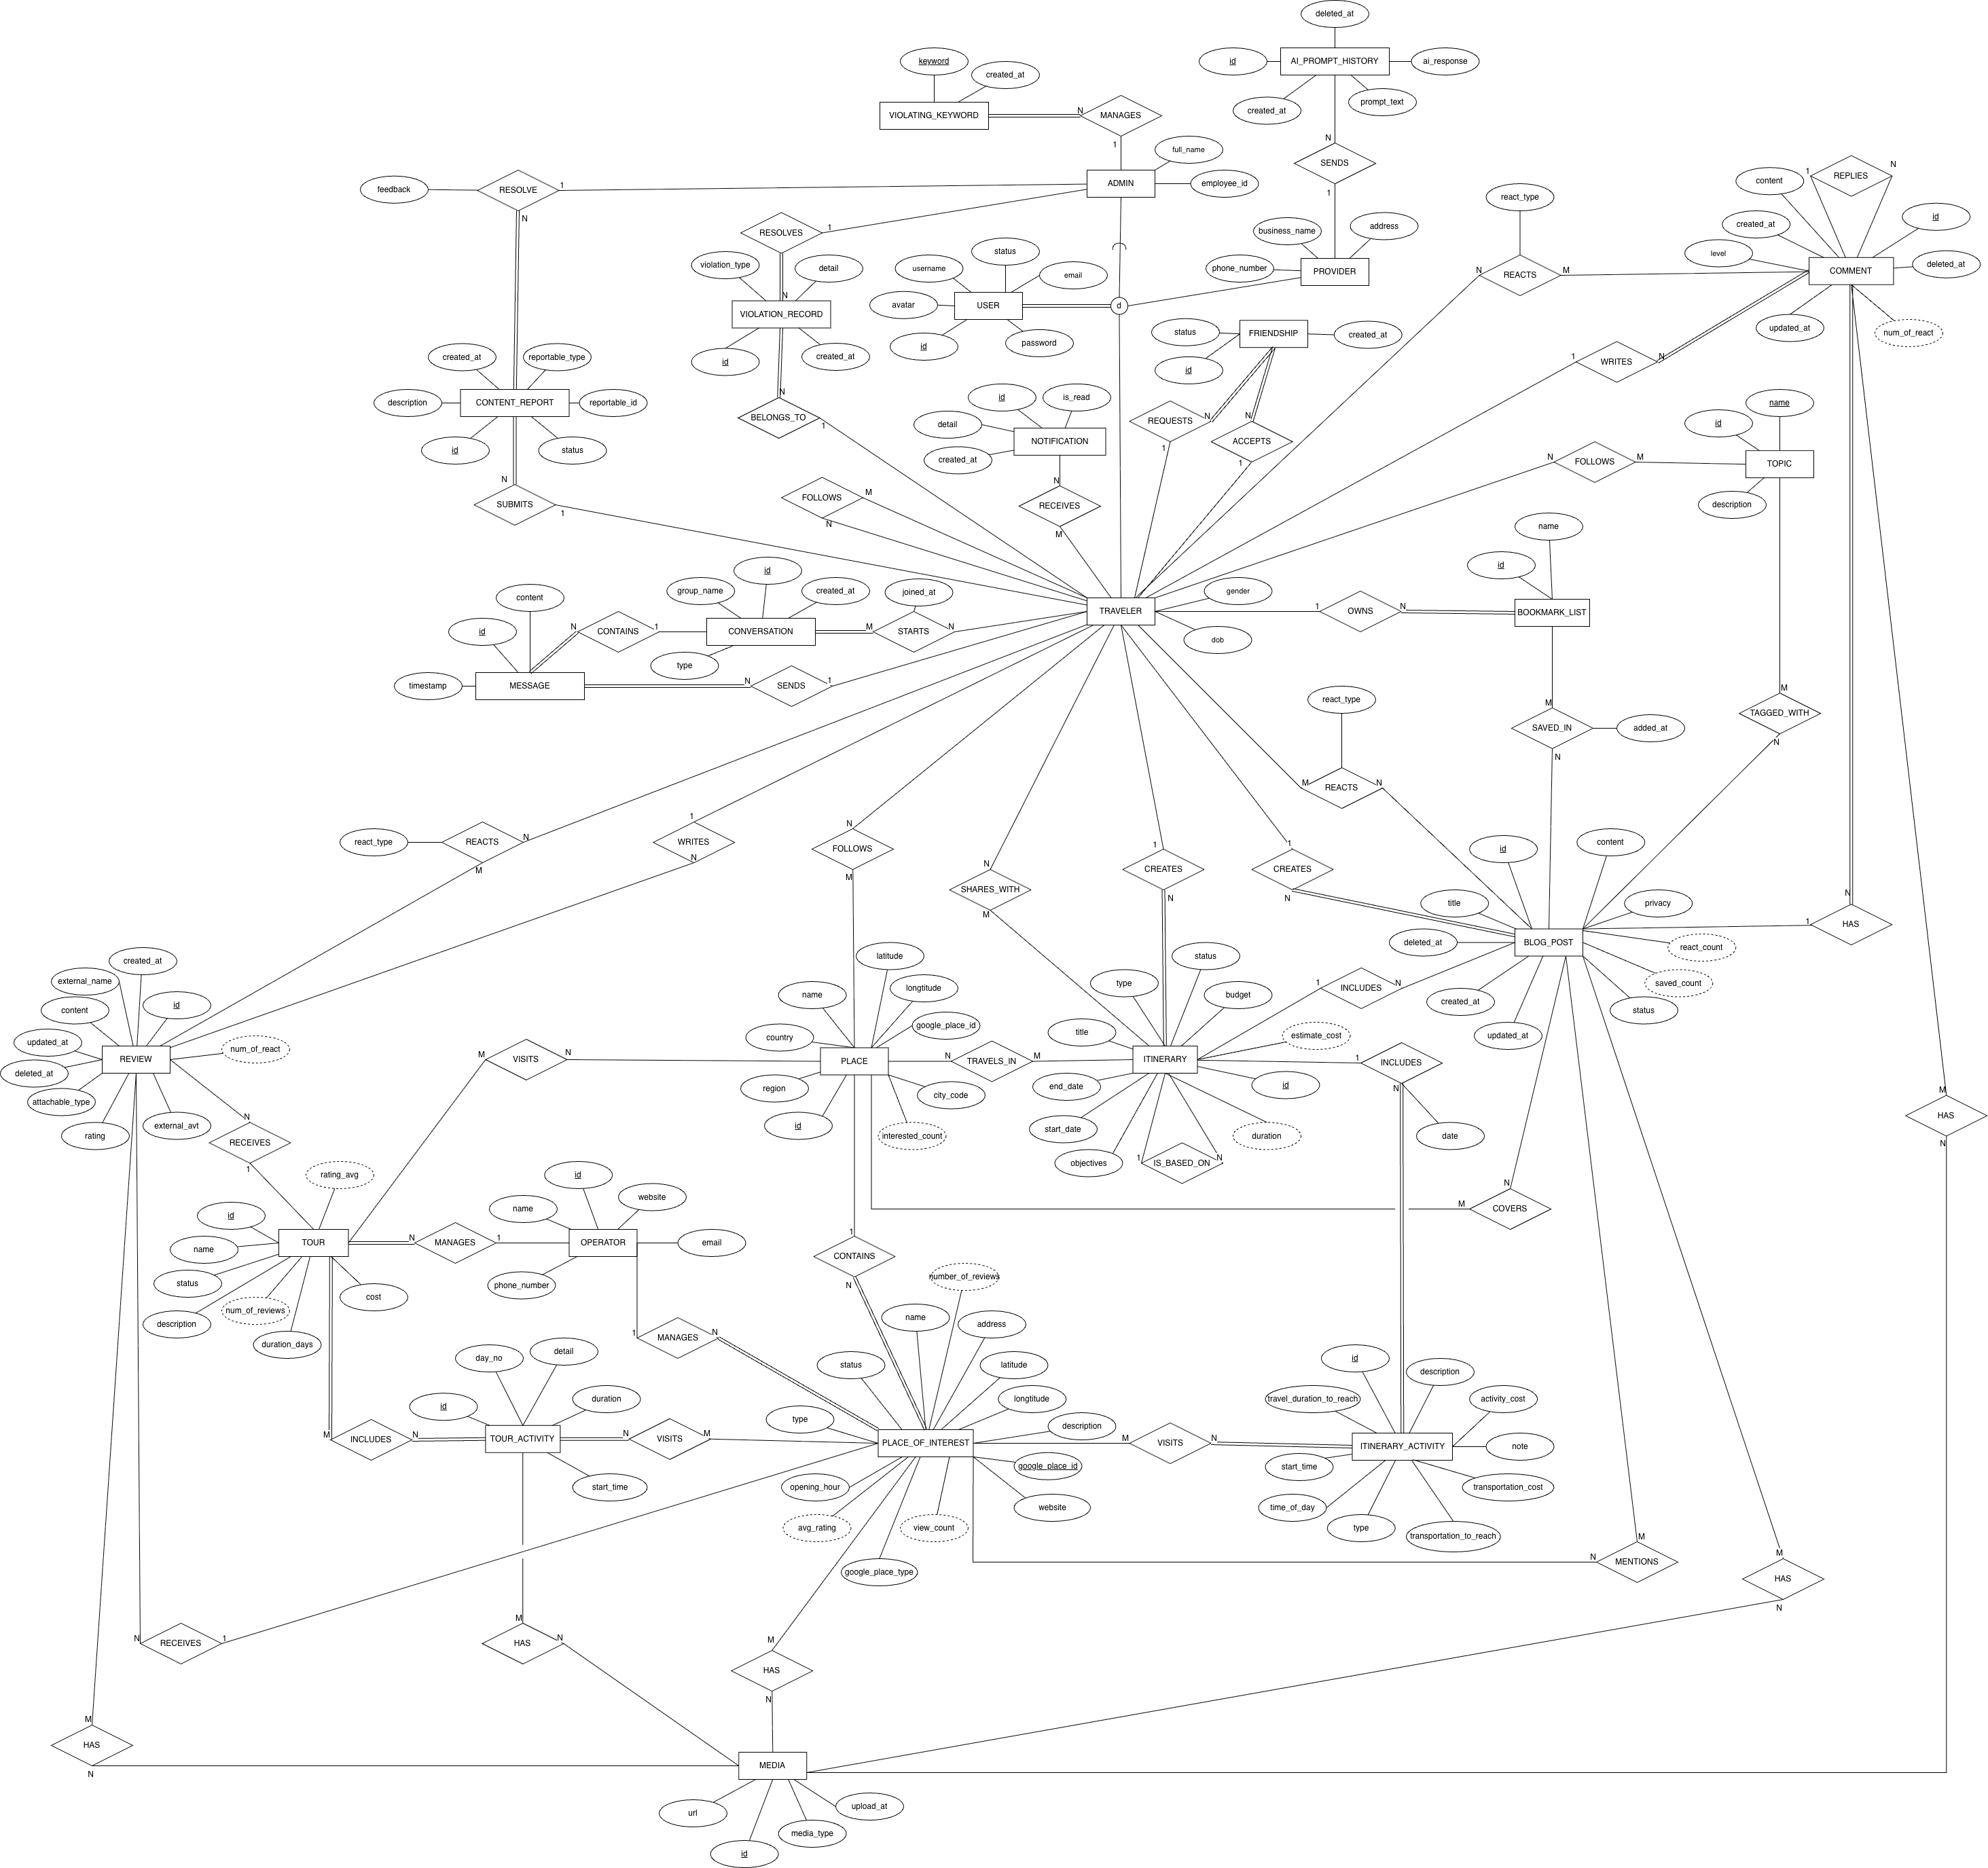
\includegraphics[width=1.1\textwidth]{Images/5. Recommend system/EERD.png}
    \caption{Thiết kế lược đồ EERD của hệ thống}
    \label{fig:eerd} 
\end{figure}  
\end{landscape}

\subsubsubsection{Thiết kế luận lý}
Sau khi đã xác định được các thực thể và mối quan hệ ở mức ý niệm, giai đoạn thiết kế luận lý tập trung vào việc chuyển đổi sơ đồ EERD thành một lược đồ cơ sở dữ liệu cụ thể, phù hợp với mô hình dữ liệu đã chọn cho TravelEZ.

Trong phần này, nhóm thực hiện việc ánh xạ các thực thể thành các bảng, xác định rõ các khóa chính, khóa ngoại và các ràng buộc dữ liệu. Mục tiêu là tạo ra một cấu trúc lưu trữ tối ưu, đảm bảo tính nhất quán của dữ liệu và tuân thủ các quy tắc chuẩn hóa để giảm thiểu dư thừa dữ liệu trong quá trình vận hành hệ thống gợi ý du lịch.

\begin{landscape}
\begin{figure}[htp]
    \centering
    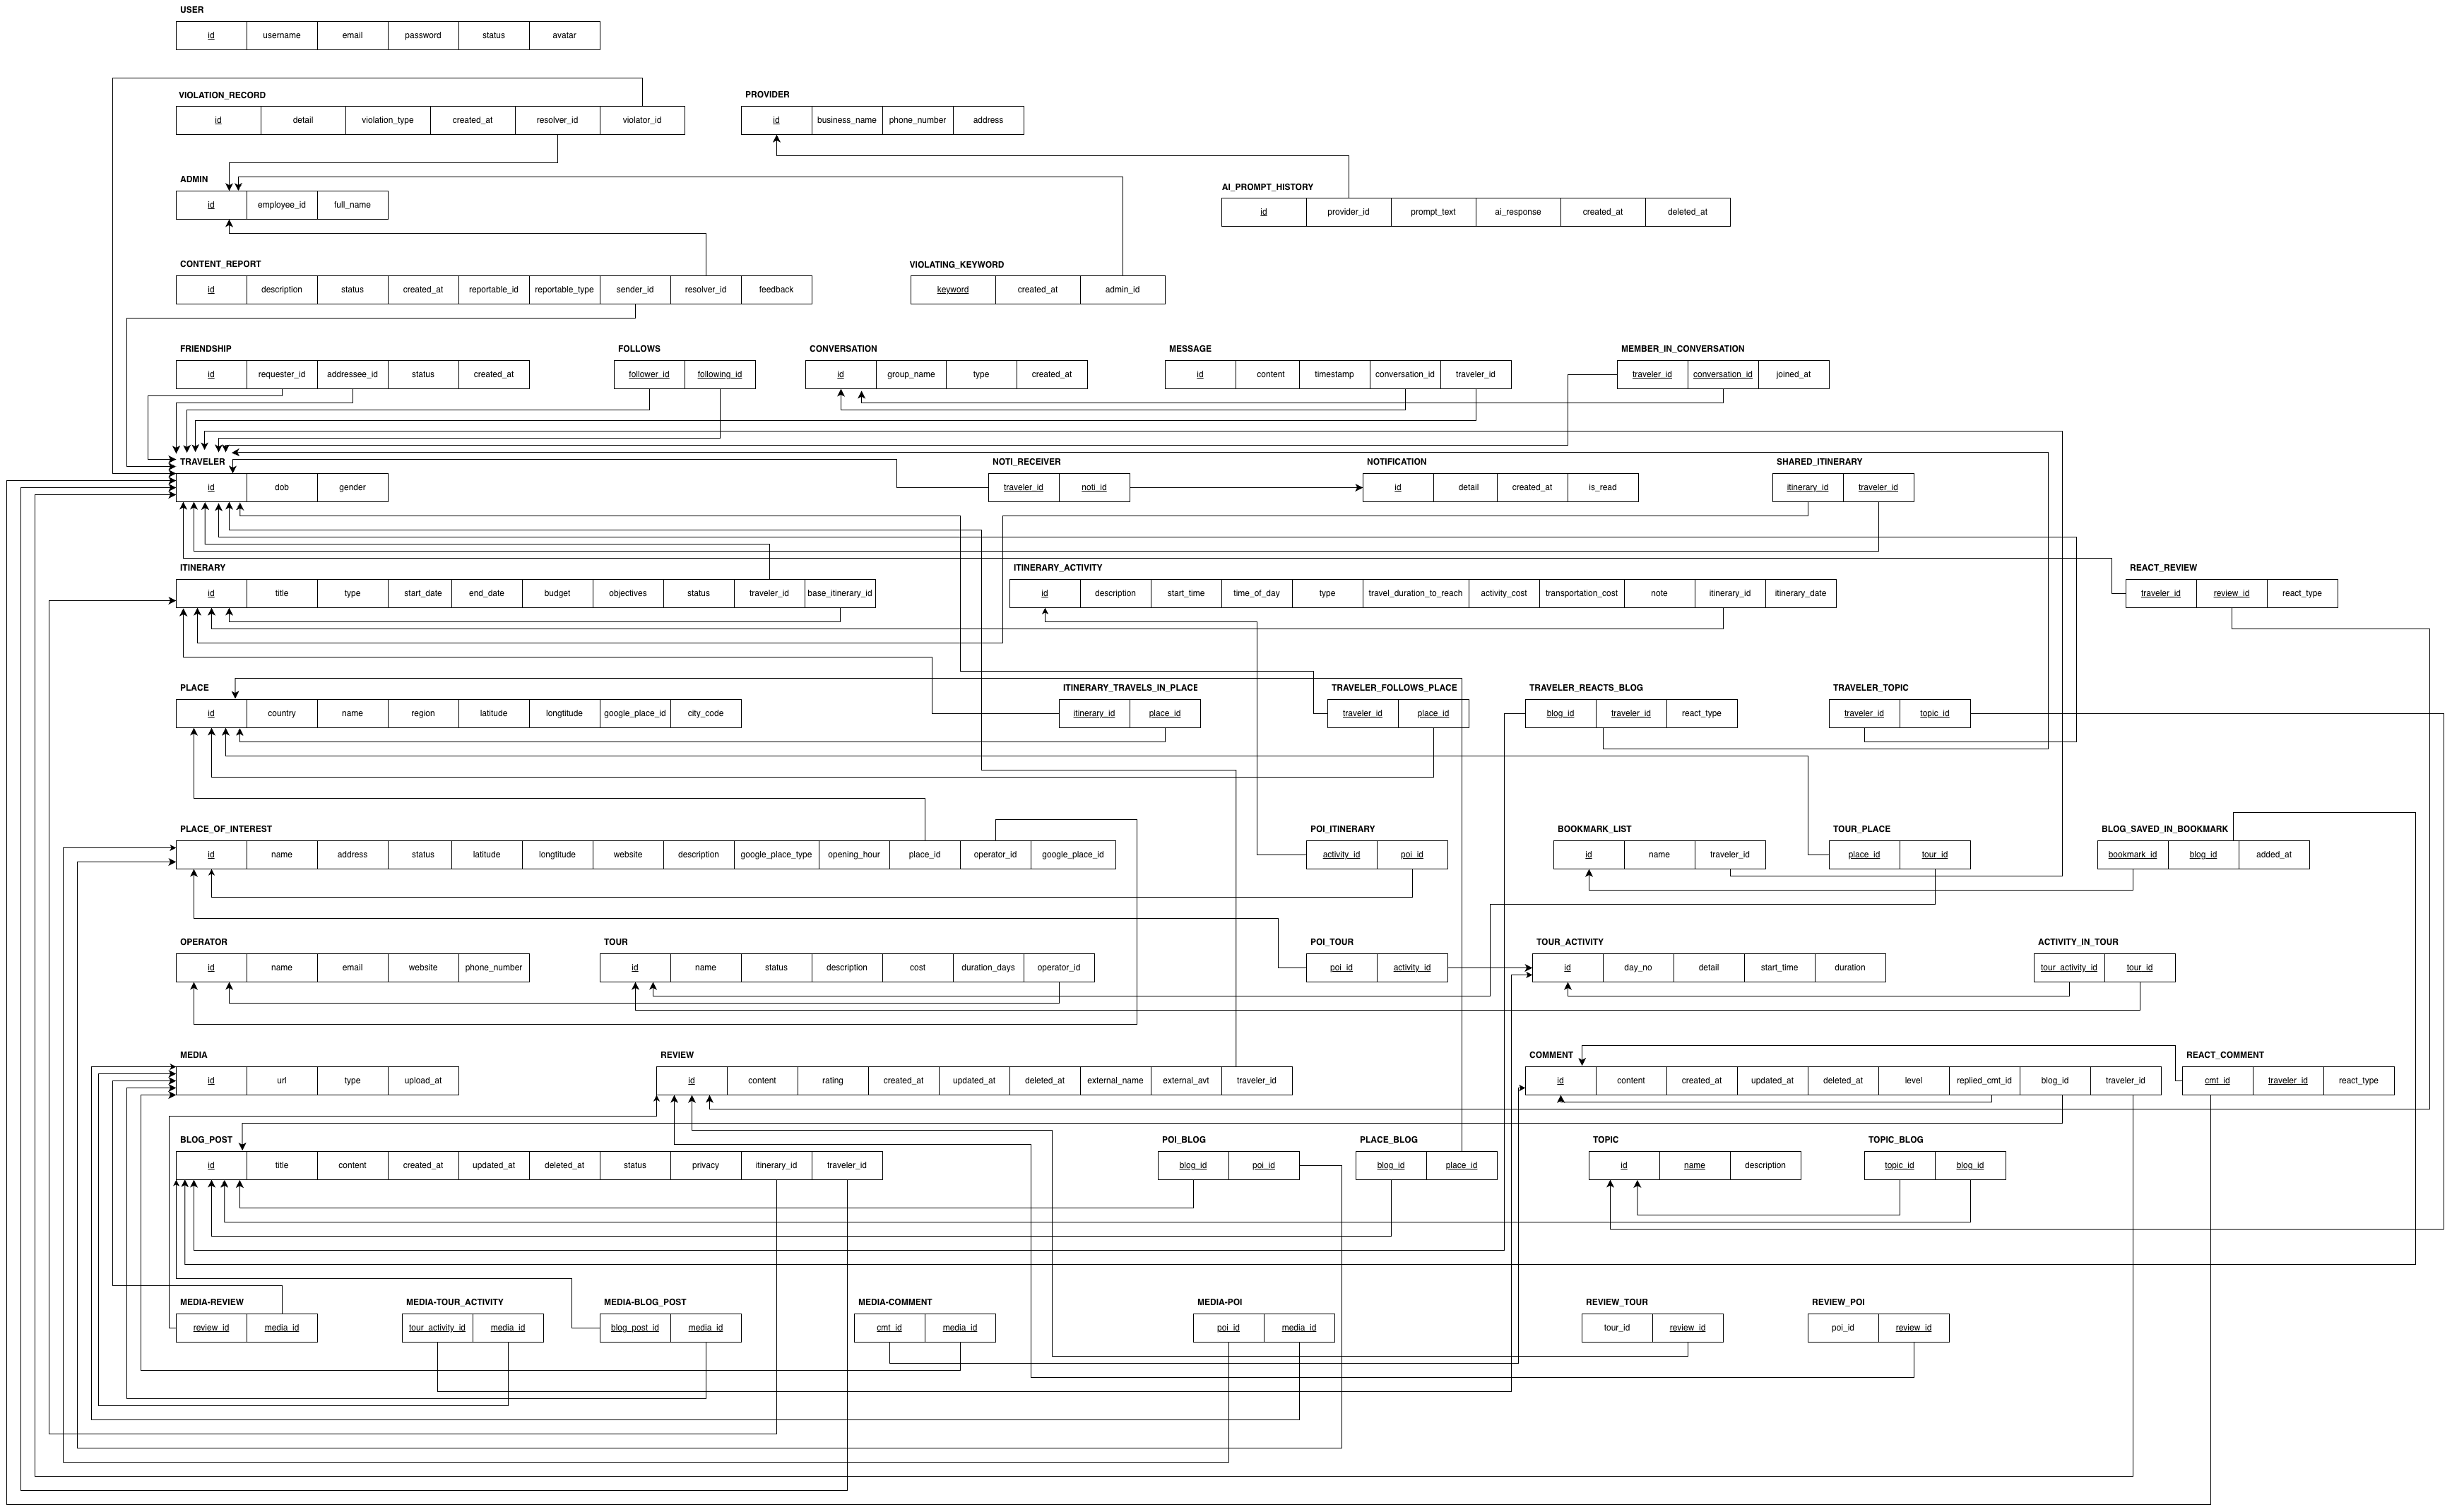
\includegraphics[width=1.5\textwidth]{Images/7. System Design/EERD-mapping.png}
    \caption{Lược đồ cơ sở dữ liệu luận lý}
    \label{fig:eerd-mapping} 
\end{figure}  
\end{landscape}


\subsubsubsection{Thiết kế vật lý}
Dưới đây là chi tiết thiết kế vật lý một số bảng quan trọng trong hệ thống. Mỗi bảng thể hiện rõ các thuộc tính, kiểu dữ liệu cụ thể, các ràng buộc và khóa ngoại (nếu có).

{\small
\begin{longtable}{|p{2.5cm}|p{3.2cm}|p{4.5cm}|p{4.3cm}|}
\caption{Thiết kế vật lý cơ sở dữ liệu}\label{tab:physical-data}\\
\hline
\textbf{Tên bảng} & \textbf{Tên thuộc tính} & \textbf{Kiểu dữ liệu} & \textbf{Ràng buộc} \\ \hline
\endfirsthead

\multicolumn{4}{c}%
{\tablename\ \thetable\ -- \textit{Tiếp theo trang trước}} \\
\hline
\textbf{Tên bảng} & \textbf{Tên thuộc tính} & \textbf{Kiểu dữ liệu} & \textbf{Ràng buộc} \\ \hline
\endhead

\hline \multicolumn{4}{r}{\textit{}} \\
\endfoot

\hline
\endlastfoot

\multirow{6}{2.5cm}{\textbf{user}} 
    & id & BIGINT & PK, NOT NULL \\ \cline{2-4} 
    & username & VARCHAR(100) & NOT NULL, UNIQUE \\ \cline{2-4} 
    & password & VARCHAR(255) & NOT NULL \\ \cline{2-4} 
    & status & ENUM('active', 'inactive') & NOT NULL, DEFAULT 'active' \\ \cline{2-4} 
    & email & VARCHAR(255) & NOT NULL, UNIQUE \\ \cline{2-4} 
    & avatar & VARCHAR(255) & \\ \hline

\multirow{3}{2.5cm}{\textbf{admin}} 
    & id & BIGINT & PK, NOT NULL \\ \cline{2-4} 
    & employee\_id & BIGINT & NOT NULL, UNIQUE \\ \cline{2-4} 
    & full\_name & VARCHAR(255) & NOT NULL \\ \hline

\multirow{4}{2.5cm}{\textbf{provider}} 
    & id & BIGINT & PK, NOT NULL \\ \cline{2-4} 
    & business\_name & VARCHAR(255) & NOT NULL \\ \cline{2-4} 
    & phone\_number & VARCHAR(20) & \\ \cline{2-4} 
    & address & VARCHAR(255) & \\ \hline

\multirow{3}{2.5cm}{\textbf{traveler}} 
    & id & BIGINT & PK, NOT NULL \\ \cline{2-4} 
    & dob & DATE & \\ \cline{2-4} 
    & gender & VARCHAR(10) & \\ \hline

\multirow{10}{2.5cm}{\textbf{itinerary}} 
    & id & BIGINT & PK, NOT NULL \\ \cline{2-4} 
    & title & VARCHAR(255) & NOT NULL \\ \cline{2-4} 
    & type & VARCHAR(255) & NOT NULL \\ \cline{2-4} 
    & start\_date & DATE & NOT NULL \\ \cline{2-4} 
    & end\_date & DATE & NOT NULL \\ \cline{2-4} 
    & budget & DECIMAL(12, 2) & NULL \\ \cline{2-4} 
    & objectives & TEXT & NULL \\ \cline{2-4} 
    & status & ENUM('planning', 'ongoing', 'completed', 'cancelled') & NOT NULL, DEFAULT 'planning' \\ \cline{2-4} 
    & traveler\_id & BIGINT & NOT NULL, FK REFERENCES traveler(id) \\ \cline{2-4} 
    & base\_itinerary\_id & BIGINT & NULL, FK REFERENCES itinerary(id) \\ \hline

\multirow{11}{2.5cm}{\textbf{itinerary\_\newline activity}} 
    & id & BIGINT & PK, NOT NULL \\ \cline{2-4} 
    & description & TEXT & \\ \cline{2-4} 
    & start\_time & TIME & \\ \cline{2-4} 
    & time\_of\_day & VARCHAR(50) & \\ \cline{2-4} 
    & type & VARCHAR(50) & \\ \cline{2-4} 
    & travel\_duration\_\newline to\_reach & INT & \\ \cline{2-4} 
    & activity\_cost & DECIMAL(10, 2) & \\ \cline{2-4} 
    & transportation\_cost & DECIMAL(10, 2) & \\ \cline{2-4} 
    & note & TEXT & \\ \cline{2-4} 
    & itinerary\_id & BIGINT & NOT NULL, FK REFERENCES itinerary(id) \\ \cline{2-4} 
    & itinerary\_date & DATE & NOT NULL \\ \hline

\multirow{8}{2.5cm}{\textbf{place}} 
    & id & BIGINT & PK, NOT NULL \\ \cline{2-4} 
    & country & VARCHAR(100) & \\ \cline{2-4} 
    & name & VARCHAR(255) & NOT NULL \\ \cline{2-4} 
    & region & VARCHAR(100) & \\ \cline{2-4} 
    & latitude & DECIMAL(10, 8) & \\ \cline{2-4} 
    & longtitude & DECIMAL(11, 8) & \\ \cline{2-4} 
    & google\_place\_id & VARCHAR(255) & NULL, UNIQUE \\ \cline{2-4} 
    & city\_code & VARCHAR(50) & \\ \hline

\multirow{13}{2.5cm}{\textbf{place\_of\_\newline interest}} 
    & id & BIGINT & PK, NOT NULL \\ \cline{2-4} 
    & name & VARCHAR(255) & NOT NULL \\ \cline{2-4} 
    & address & VARCHAR(255) & \\ \cline{2-4} 
    & status & ENUM('operational', 'temporarily\_closed', 'permanently\_closed') & NOT NULL, DEFAULT 'operational' \\ \cline{2-4} 
    & latitude & DECIMAL(10, 8) & \\ \cline{2-4} 
    & longtitude & DECIMAL(11, 8) & \\ \cline{2-4} 
    & website & VARCHAR(255) & \\ \cline{2-4} 
    & description & TEXT & \\ \cline{2-4} 
    & google\_place\_type & VARCHAR(100) & \\ \cline{2-4} 
    & opening\_hour & TEXT & \\ \cline{2-4} 
    & place\_id & BIGINT & NOT NULL, FK REFERENCES place(id) \\ \cline{2-4} 
    & operator\_id & BIGINT & NULL, FK REFERENCES operator(id) \\ \cline{2-4} 
    & google\_place\_id & VARCHAR(255) & NULL, UNIQUE \\ \hline

\multirow{10}{2.5cm}{\textbf{blog\_post}} 
    & id & BIGINT & PK, NOT NULL \\ \cline{2-4} 
    & title & VARCHAR(255) & NOT NULL \\ \cline{2-4} 
    & content & LONGTEXT & \\ \cline{2-4} 
    & status & ENUM('draft', 'published', 'archived') & NOT NULL, DEFAULT 'draft' \\ \cline{2-4} 
    & privacy & ENUM('public', 'friends\_only', 'private') & NOT NULL, DEFAULT 'public' \\ \cline{2-4} 
    & created\_at & TIMESTAMP & NOT NULL, DEFAULT CURRENT\_TIMESTAMP \\ \cline{2-4} 
    & deleted\_at & TIMESTAMP & \\ \cline{2-4} 
    & updated\_at & TIMESTAMP & \\ \cline{2-4} 
    & itinerary\_id & BIGINT & NULL, FK REFERENCES itinerary(id) \\ \cline{2-4} 
    & traveler\_id & BIGINT & NOT NULL, FK REFERENCES traveler(id) \\ \hline

\end{longtable}
}

\subsubsubsection{Truy vấn với Index}
Nhóm đã phân tích các luồng nghiệp vụ chính và xác định các cột thường xuyên được sử dụng trong các mệnh đề WHERE, JOIN và ORDER BY để tạo các chỉ mục phù hợp. Bảng dưới đây trình bày một số index tiêu biểu đã được triển khai và vai trò của chúng trong hệ thống.
\begin{longtable}{|p{7cm}|p{7cm}|}
    \caption{Mô tả một số Index tiêu biểu trong thiết kế vật lý}\\
    \hline
    \textbf{Tên Index} & \textbf{Mục đích \& Tác động} \\
    \hline
    \endfirsthead
    
    \caption{Mô tả một số Index tiêu biểu trong thiết kế vật lý}\\
    \hline
    \textbf{Tên Index} & \textbf{Mục đích \& Tác động} \\ \hline
    \endhead
    \hline
    \endlastfoot

    \textbf{idx\_users\_fullname\_lower} & Tăng tốc độ tìm kiếm thông tin người dùng qua họ tên. Đây là thao tác thường xuyên khi người dùng tìm kiếm bạn bè hoặc chuyên gia trên thanh công cụ tìm kiếm của hệ thống. \\ \hline
    \textbf{idx\_posts\_status\_created} & Phục vụ truy vấn lấy danh sách bài đăng trên trang chủ (Newsfeed). Index composite này giúp hệ thống lọc nhanh các bài viết ở trạng thái PUBLISHED và sắp xếp theo thời gian mới nhất một cách tối ưu. \\ \hline
    \textbf{idx\_poi\_place\_type\_status} & Tối ưu hóa các truy vấn tìm kiếm, lọc địa điểm tham quan (POI) theo khu vực (place\_id), loại hình (poi\_type) và trạng thái. Rất quan trọng cho tính năng bản đồ, khám phá và gợi ý điểm đến. \\ \hline
    \textbf{idx\_itinerary\_traveler\_status} & Tối ưu hóa việc truy xuất danh sách lịch trình chuyến đi của một du khách (traveler\_id) theo trạng thái (đang lên kế hoạch, đang đi, đã hoàn thành). Giúp trang quản lý chuyến đi cá nhân tải dữ liệu nhanh chóng. \\ \hline  
    \textbf{idx\_comment\_post\_created} & Hỗ trợ truy vấn tải danh sách bình luận của một bài đăng cụ thể. Tránh việc hệ thống phải quét toàn bộ bảng comment, đồng thời hỗ trợ sắp xếp thứ tự bình luận theo thời gian một cách mượt mà. \\ \hline
    \textbf{idx\_follow\_following\_id} & Phục vụ truy vấn lấy danh sách "Người theo dõi" (Followers) của một cá nhân. Do khóa chính (follower\_id, following\_id) chỉ hỗ trợ tốt chiều tìm "Đang theo dõi", index này bắt buộc phải có để tối ưu chiều ngược lại. \\ \hline
    \textbf{idx\_message\_conv\_created} & Tăng tốc các truy vấn tải lịch sử tin nhắn trong một hộp thoại cụ thể, thường xuyên dùng kết hợp với ORDER BY trong màn hình chat để luôn hiển thị các tin nhắn mới nhất lên trước. \\ \hline
\end{longtable}
